\documentclass[11pt]{article}
\usepackage[margin=1in]{geometry}
\usepackage{graphicx,booktabs,amsmath}
\usepackage[numbers]{natbib}
\usepackage[hidelinks]{hyperref}


\title{AURORA: An Auditable Protocol and DCGAN Execution Feasibility Study}
\author{Rayan Rahman\\Marathwada Mitra Mandal Institute of Technology}
\date{Working draft: November 2026}

\begin{document}
\maketitle

\begin{abstract}
Synthetic image augmentation offers a potentially testable approach to mitigate scarcity in labeled chest radiograph datasets for tuberculosis (TB) screening. We present AURORA, an auditable research pipeline and prospective protocol for synthetic TB radiograph augmentation. From an initial inventory of 800 images from the Shenzhen and Montgomery collections, an automated similarity-based exclusion process removed 210 images involved in flagged similarity pairs, resulting in a final subset of 590 images (289 normal, 301 TB-labelled). We report feasibility results for a bounded execution run: a two-epoch Deep Convolutional Generative Adversarial Network (DCGAN) training session on an NVIDIA RTX 4050 Laptop GPU. The run achieved a trainer runtime of 1.32s and peak PyTorch allocated memory of 216.92 MiB. This report establishes bounded execution feasibility and protocol auditability; downstream predictive utility and clinical validation of the synthetic outputs have not yet been executed.
\end{abstract}

\section{Introduction}
Synthetic radiographs provide a testable method for augmenting limited labeled training sets in medical imaging. However, an informative experiment must strictly distinguish between nominal oversampling and the specific benefits introduced by a learned generator. Generator execution feasibility and downstream predictive utility are separate questions. AURORA addresses this by establishing an auditable research pipeline and a prospective four-condition protocol using TB-manifestation-labelled chest radiographs from the Shenzhen and Montgomery collections \cite{jaeger2014}.

The scarcity of positive cases in this study is imposed experimentally by limiting positive training images while keeping normal training images fixed, rather than representing true population prevalence. AURORA contributes a documented dataset selection process, a hash-bound execution protocol, and a prospective count-matched experimental design. The current work focuses on a measured feasibility run to ensure training provenance and execution stability within a bounded budget, rather than claiming architectural novelty or clinical superiority.

\section{Related Work}
\subsection{Generative Models for Medical Imaging}
Generative Adversarial Networks, specifically the DCGAN architecture \cite{radford2015}, provide a convolutional baseline for adversarial image learning. While DCGANs are widely used, their standard implementations may fail to preserve specific radiographic features or anatomical plausibility without domain-specific constraints. Recent advancements have explored adapted latent diffusion models for pathological analysis in chest X-rays \cite{moris2024}, which offer different trade-offs in fidelity and diversity compared to GAN-based approaches. AURORA adopts DCGAN as a baseline but prioritizes an auditable execution protocol to ensure training provenance over architectural complexity.

\subsection{Synthetic Augmentation Evaluation Frameworks}
A critical challenge in synthetic augmentation is disentangling the effects of increased dataset size from the diversity introduced by the generator. Research by \citet{pink2026} suggests that superior generative metrics, such as the Fréchet Inception Distance (FID), do not consistently translate to improved downstream classifier performance when compared to count-matched real duplication. Furthermore, systematic reviews of synthetic medical imaging highlight heterogeneous evaluation methods and limitations in reproducibility and bias assessment \cite{folguera2026}. AURORA’s prospective protocol explicitly includes count-matched real duplication and conventional augmentation as essential comparators to isolate the utility of synthetic data.

\section{Materials and Implemented Methods}

\subsection{Dataset Selection}
The study utilizes the Shenzhen and Montgomery chest X-ray collections \cite{jaeger2014}. The initial inventory consisted of 800 images (406 normal, 394 TB-labelled). Using a predefined selection rule, we performed an automated similarity-based exclusion of 210 images involved in 206 flagged similarity pairs. This resulted in 590 retained images. The final stratified split, detailed in Table 1, allocated 413 images for training, 89 for validation, and 88 for testing. We acknowledge that differential exclusion rates between cohorts (30.06\% for Shenzhen vs. 7.97\% for Montgomery) introduce potential selection bias.

\begin{table}[ht]
\centering
\caption{Image-level selection and split counts across cohorts and labels.}
\label{tab:dataset_split}
\begin{tabular}{lrrrrrr}
\toprule
Cohort and label & Original & Excluded & Retained & Train & Validation & Test \\
\midrule
Shenzhen normal & 326 & 112 & 214 & 150 & 32 & 32 \\
Shenzhen TB-labelled & 336 & 87 & 249 & 174 & 38 & 37 \\
Montgomery normal & 80 & 5 & 75 & 53 & 11 & 11 \\
Montgomery TB-labelled & 58 & 6 & 52 & 36 & 8 & 8 \\
\midrule
Total & 800 & 210 & 590 & 413 & 89 & 88 \\
\bottomrule
\end{tabular}
\end{table}

\subsection{Preprocessing and Access Control}
Images were resized to $128 \times 128$ pixels, converted to grayscale, and normalized to the $[-1, 1]$ range. A v2 approval gate was implemented to bind seven artifacts—including configuration, protocol, and dataset manifests—via SHA-256 hashes. This protocol ensures that the image reader rejects non-selected IDs and verifies hashes before decoding, rejecting access to nonselected image IDs before reading bytes. This is an application-level control around trusted code, not an operating-system sandbox or evidence of patient independence. A prefix-based budget system was established for TB training images at 25\% (52 images), 50\% (105 images), and 100\% (210 images) levels.

\subsection{Bounded DCGAN Configuration}
The DCGAN architecture follows the design by \citet{radford2015}, with a latent dimension of 100 and generator/discriminator widths of 64. Optimization used the Adam optimizer with a learning rate of 0.0002 and $\beta$ values of 0.5 and 0.999. For the feasibility run, we used a batch size of 16 and trained for 2 epochs in full precision, with batches of 16/16/16/4 and one discriminator update per generator update. Epoch losses are arithmetic means of batch losses, including the smaller final batch. The final checkpoint passed epoch/configuration checks; no validation/test images were read and no classifier was trained. Real discriminator targets were smoothed to 0.9, while fake targets were set to 0.0.

\section{Measured Feasibility Results}

\subsection{Execution Metrics}
The feasibility run was conducted on an NVIDIA GeForce RTX 4050 Laptop GPU. The trainer runtime was recorded at 1.32s, with a peak PyTorch allocated memory of 216.92 MiB. Entry-function total runtime excludes interpreter/import startup; trainer timing includes checkpoint and sample output. Memory values describe the PyTorch allocator, not total device usage. Only one run was timed. The execution workflow is illustrated in Figure 1.

\begin{figure}[ht]
\centering
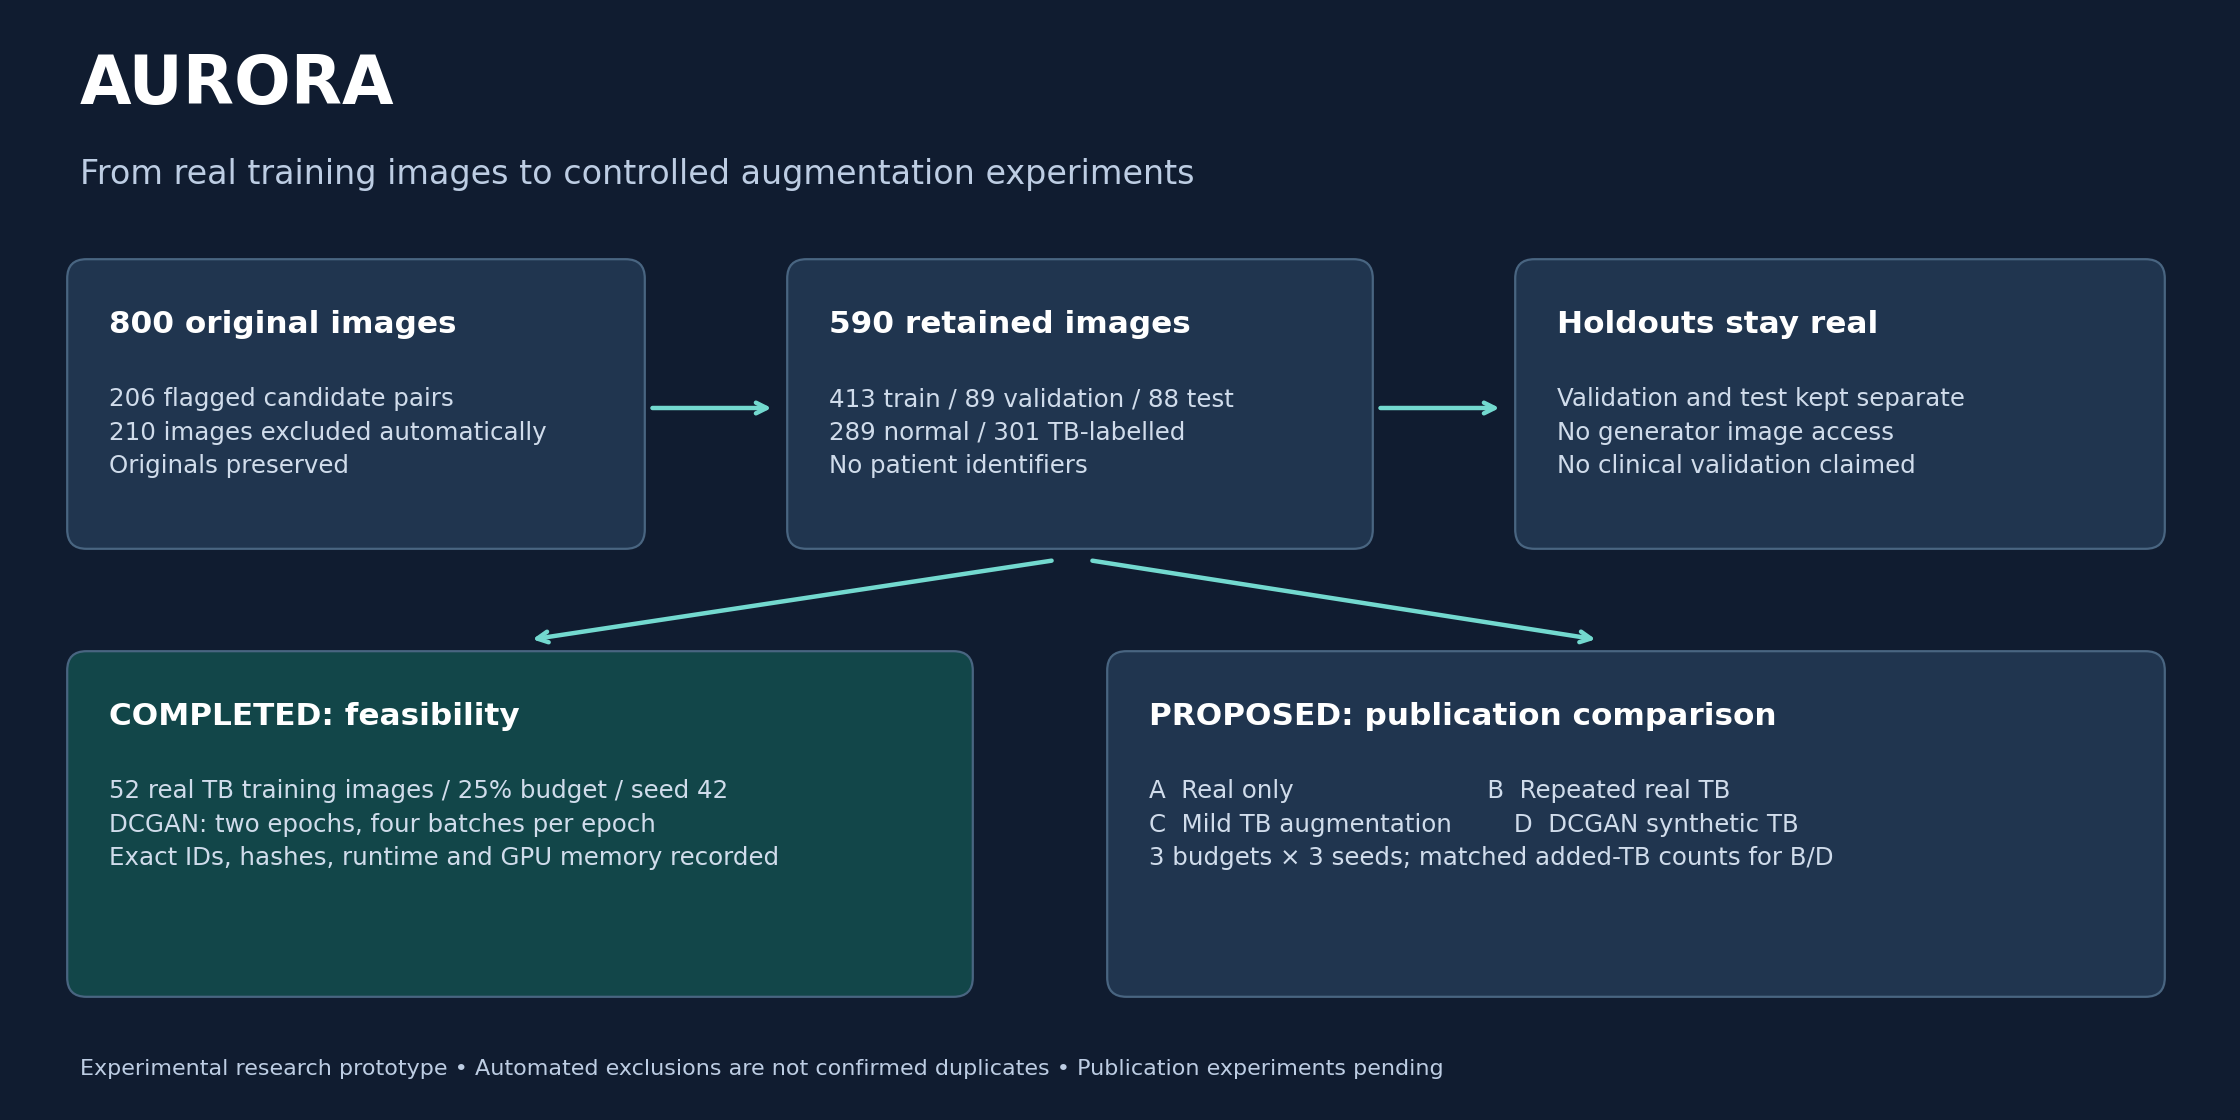
\includegraphics[width=0.8\textwidth]{../../../docs/images/aurora-workflow.png}
\caption{Schematic of automated image selection, fixed image-level split, completed feasibility run and proposed unexecuted four-condition comparison. Counts are images, not unique patients.}
\label{fig:workflow}
\end{figure}

\subsection{Training Loss Observations}
The generator and discriminator losses were monitored over the two-epoch run. The generator loss decreased from 0.618 to 0.487, while the discriminator loss decreased from 0.391 to 0.192. These metrics are summarized in Table 2 and visualized in Figure 2. Recorded read IDs confirmed that only the approved 52-source prefix was accessed, with zero holdout overlap.

\begin{table}[ht]
\centering
\caption{Single-run feasibility measurements on NVIDIA RTX 4050.}
\label{tab:feasibility_metrics}
\begin{tabular}{lr}
\toprule
Measurement & Observed Value \\
\midrule
Trainer runtime & 1.3219 s \\
Entry-function total runtime & 6.1937 s \\
Peak PyTorch allocated GPU memory & 216.92 MiB \\
Peak PyTorch reserved GPU memory & 282.00 MiB \\
Generator mean loss (Epoch 1 / 2) & 0.6178 / 0.4872 \\
Discriminator mean loss (Epoch 1 / 2) & 0.3908 / 0.1918 \\
\bottomrule
\end{tabular}
\end{table}

\begin{figure}[ht]
\centering
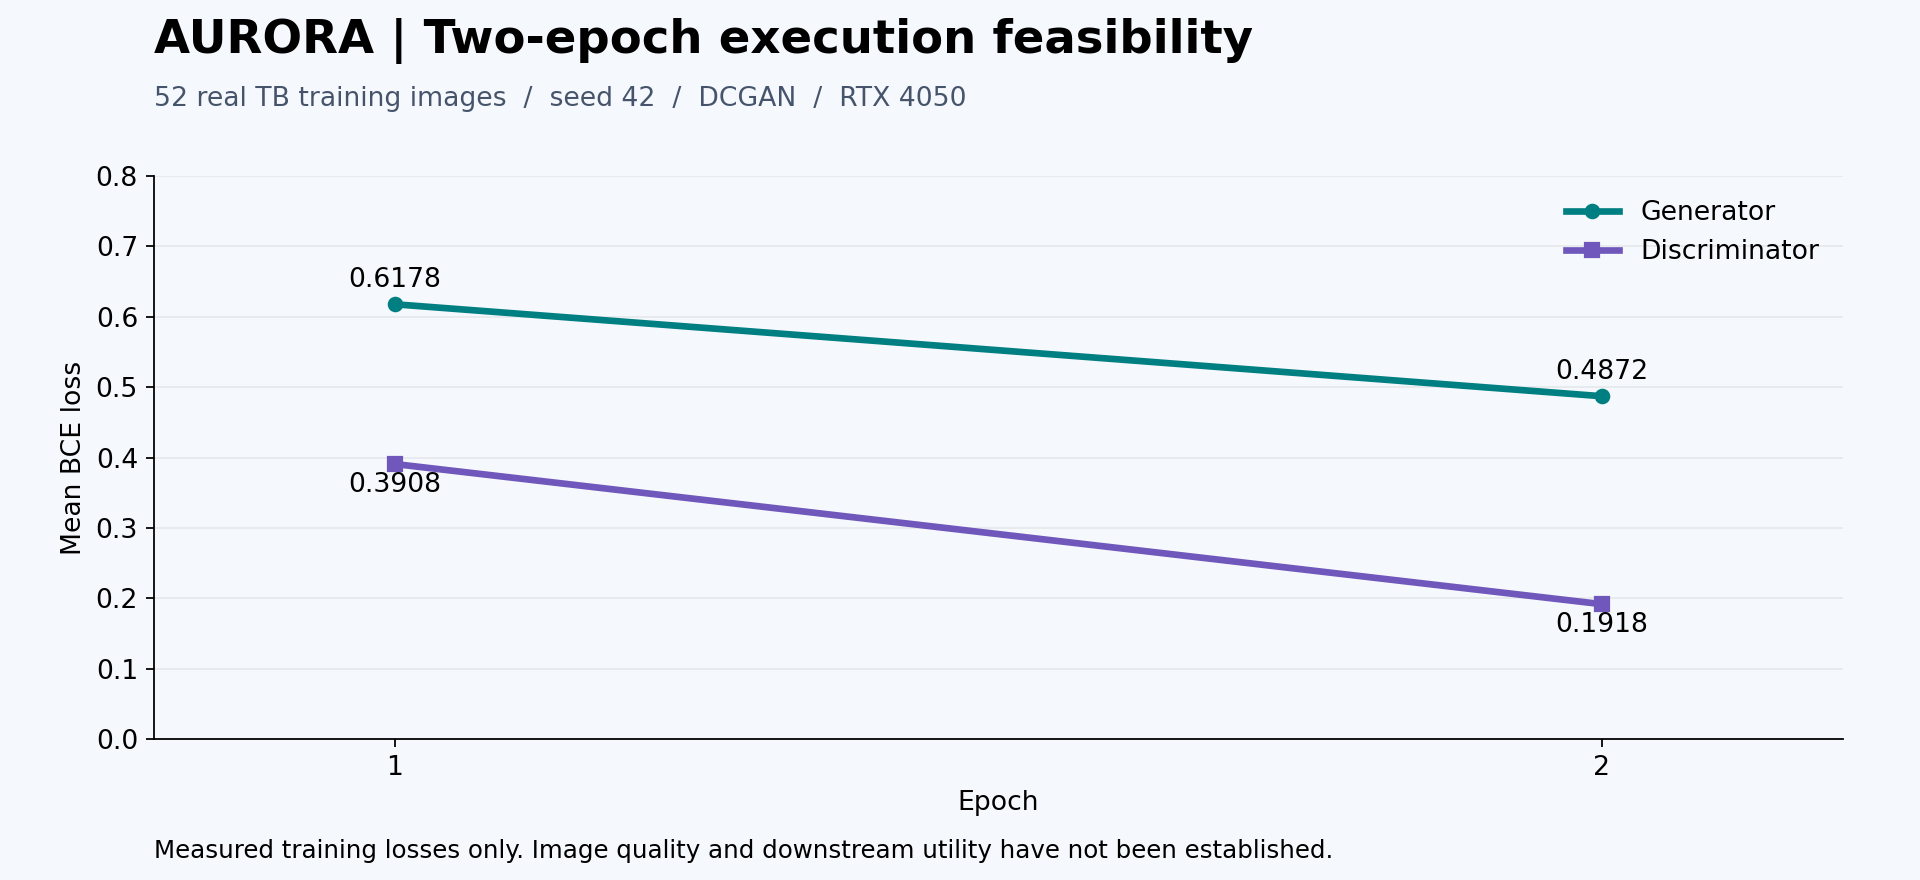
\includegraphics[width=0.8\textwidth]{../../../docs/images/feasibility-losses.png}
\caption{Measured batch-mean generator and discriminator losses for two epochs, 52 real TB training images, seed 42. Not evidence of convergence or clinical image quality.}
\label{fig:losses}
\end{figure}

\section{Prospective Comparison: Not Executed}

\subsection{Proposed Experimental Design}
The planned study compares four conditions:
\begin{itemize}
    \item \textbf{Condition A}: Real images only.
    \item \textbf{Condition B}: Real duplication (Condition A plus repeated real TB images).
    \item \textbf{Condition C}: Conventional transforms applied only to TB training images: rotation up to 5 degrees, translation up to 5 percent, brightness/contrast jitter 0.1, and no horizontal flips.
    \item \textbf{Condition D}: Synthetic augmentation (Condition A plus DCGAN-generated TB images).
\end{itemize}

The proposed classifier is a ResNet-18 model pretrained on ImageNet, optimized using Adam with a 1,000-update budget. TB recall is the primary endpoint; AUPRC, F1, specificity and AUROC are supporting outcomes. B and D add exactly 52, 105 or 210 TB images at their respective budgets. Three budgets and seeds 42/123/999 imply 36 classifier fits and nine GAN fits, none yet executed. The separate v2 publication runner still requires integration and authorization. The full GAN training duration for the effectiveness study is set to 200 epochs.

\section{Discussion and Limitations}
The AURORA protocol ensures provenance through hash-bound access, but it does not guarantee patient independence due to the lack of unique patient identifiers in the source datasets. The small subgroup sizes in the Montgomery collection mean that cohort-specific results will be descriptive rather than statistically robust. Furthermore, the low resolution ($128 \times 128$) and the absence of clinical validation for synthetic outputs limit the current diagnostic interpretation. The feasibility run demonstrates that the workflow executes correctly on consumer-grade hardware, but it does not yet establish the clinical utility of the generated images.

The exclusions are not confirmed duplicates; retained images may still include repeated patients or transformed duplicates. A single error among eight Montgomery TB test images changes subgroup recall by 12.5 percentage points. No image-quality, memorization or clinical assessment has been completed.

\section{Conclusion}
This work establishes the feasibility of the AURORA protocol for auditable synthetic radiograph augmentation. One bounded DCGAN execution used only 52 real TB training images selected from the training partition of the 590-image subset. Its source identity, epoch and configuration checks passed. These checks are limited to the implemented software paths;  the impact of synthetic augmentation on TB classification performance remains an open question for future investigation.

\section*{Declarations}
\textbf{Reproducibility:} Code is available at \url{https://github.com/xt67/AURORA} under the Apache License 2.0. Configuration SHA-256: \nolinkurl{6a2b34cb819c805ba3e7523ed7ef65ef74dfb6b2c5ac9532155217e7354a950e}. Checkpoint SHA-256: \nolinkurl{6d24fb1c9750a2e9e5c61162d83f36001c86e2141e541caa29f39ec33041ee6d}.

\textbf{AI Assistance Disclosure:} This draft was prepared with assistance from Codex and the PaperOrchestra software repository \cite{paperorchestra}. The outline and writing utilized Paper Orchestra prompts via a REST adapter. The automated literature-search and full refinement pipeline were not executed. References were supplied from the curated project bibliography. Codex reviewed the generated draft against recorded evidence; final author review is still required.

\textbf{Author Confirmation:} Rayan Rahman is the sole author. Corresponding author details, contributions, funding, competing interests and applicable data-use/ethics determinations require author confirmation. No institutional approval or exemption is claimed.

\bibliographystyle{plainnat}
\bibliography{references}

\end{document}
